%describe how you evaluated to show that your approach was successful. You may need a methods section, a results section and a conclusion

This chapter reflects on the theoretical architecture (see Figure \ref{fig:wrtc-enterprise-gateway}) created in the integration chapter. I will break down each component of the gateway and test individual functionality using available open source tools. Secondly I will compare my model against a study 3GPP\footnote{http://www.3gpp.org/} did on giving \gls{wrtc} clients access to \gls{ims}, which is similar to this case. Then I will discuss the results and derive some guidelines.

\section{Evaluating the proposed gateway}
In this section a lot of experiments were conducted using sipml5\footnote{http://sipml5.org/}, which is an open-source HTML5 SIP client using \gls{rtcweb} for the media stack. It uses a SIP proxy for translating the signaling, a RTCWebBreaker to convert the media streams, and a media coder for transcoding. It operates very similar to my proposed architecture. In addition it connects to any SIP endpoint directly from the browser.

\subsection{The Signaling proxy}
In the signaling component a proxy solution was proposed to use a SIP stack for Javascript running over WebSockets. Using sipml5 and a range of different desktop SIP clients I tested to see how well the SIP proxy worked.   

\begin{table}[h]
\resizebox{\textwidth}{!}{%
\begin{tabular}{|p{1.3cm}|l|l|p{4cm}|p{4cm}|p{5cm}|}
\hline
SIP desktop clients & Audio & Video  & Latency                                                                                         & Quality                                                  & Comments                                                                                                            \\ \hline
Ekiga               & g.711 & failed & none                                                                                            & good audio quality                                       & did not get video working                                                                                           \\ \hline
Zoiper              & g.711 & vp8    & none for audio, video took approximately 5 seconds to appear, but then it was a live connection & good audio quality, huge packet loss on the video stream & crashed after just a few seconds during video conference                                                            \\ \hline
Jitsi               & g.711 & failed & none                                                                                            & good audio quality                                       & connection failed every time the application tried to negotiate a video codec, but worked fine when disabling video \\ \hline
Blink               & opus  & failed & none                                                                                            & good audio quality                                       & did not get video working                                                                                           \\ \hline
\end{tabular}
}
\caption{SIP desktop client interaction with web client using proxy and RTCWEB}
\label{tbl:sip-client-webrtc-interaction}
\end{table}

In figure \ref{tbl:sip-client-webrtc-interaction} the audio and video columns refer to the mutually agreed upon codec to be used during the signaling process. Since g.711 is the most preferred codec to be used in \gls{voip} systems, it is natural that audio most often defaults to this codec. Experiments with video conferencing was not very successful, it was difficult getting a normal video session to work for various reasons, one of them being a mismatch in the \gls{sdp} which was noted in the interoperation chapter as a probable outcome. The one desktop client that did manage to get a working video session using the VP8 codec had a very high packet loss as seen in figure \ref{fig:wireshark-sip-call}. Reasons for this is hard to say as the experiment was done on a really good connection.

\newpage
\begin{figure}[here]
\centerline{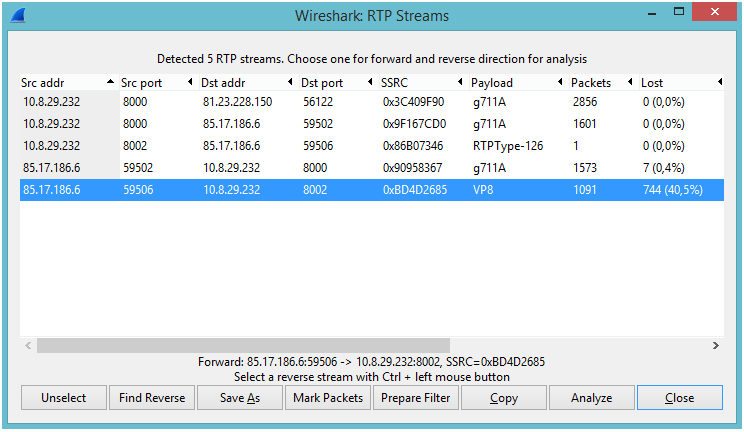
\includegraphics[scale=0.6]{wireshark-rtp.png}}
\caption{Wireshark analysis of a SIP call}
\label{fig:wireshark-sip-call}
\end{figure}

\subsection{The Transport Proxy}
Not much problems here, the connections were smooth with low latency, even running behind a proxy the connection felt `live'. As mentioned earlier there was no problems doing audio calls, but video calling seemed to cause some problems, this is probably not related to this component.

%%FYLL UT %%

\subsection{The Media Transcoder}
Since transcoding can be done in the cloud, the quality should not really be affected by this component, with todays hardware we can do live-transcoding, with little latency. Which codec used can somewhat limit latency, but the biggest latency issue has to do with the clients physical geographic location. The closer a client is to the mediaserver the better, as the media doesn't have to travel that far. 

%%FYLL UT%%

\section{Evaluate against criteria defined by 3GPP}
There is an ongoing effort at the 3GPP on giving \gls{wrtc} clients access to \gls{ims} with 3GPP TR 23.701\cite{3gpp-wrtc-access-ims} as the current proposed architecture. \gls{ims} is basically an architectural framework for delivering IP multimedia services. It was originally designed for evolving mobile networks beyond \gls{gsm}. Later it has evolved to include Wireless LAN and fixed lines, it's intended to aid the access of multimedia and voice applications across different networks. This study is relevant because most telecom companies already have IMS or a similar architecture in place for doing real-time communication. The following diagram shows the proposed architecture:

\begin{figure}[here]
\centerline{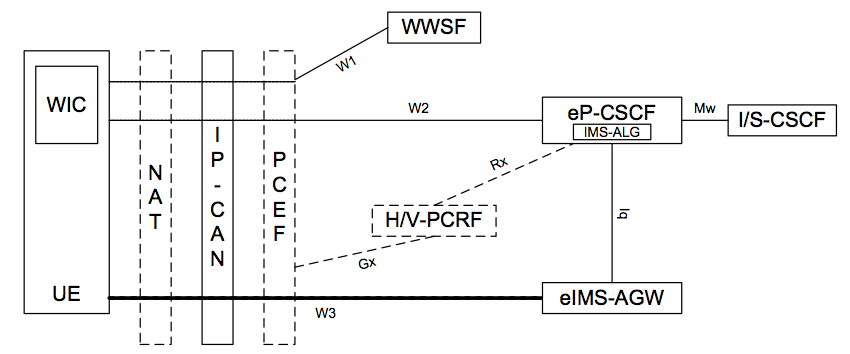
\includegraphics[scale=0.5]{3gpp-wrtc-ims-architecture.png}}
\caption{WebRTC IMS architecture by 3GPP TR 23.701 as work in progress.}
\label{fig:wrtc-ims-architecture}
\end{figure}

Let's look at the main elements:

\textbf{WebRTC IMS Client (WIC)}
is downloaded from the WWSF. It provides the application logic and \gls{wrtc} API calls to access the communication services of \gls{ims}. It works on any device supporting a browser that supports \gls{wrtc}. This is basically the same component as the mobile client in the previous chapter.

\textbf{User Equipment(UE)}
is a device or application. It can be a web application running in a browser, a tablet or mobile phone.

\textbf{WebRTC Web Server Function (WWSF)}
is from where the client is downloaded. This could be a web server hosting the WIC, or an app store such as Google Play.

\textbf{P-CSCF enhanced for WebRTC (eP-CSCF)}
is the entry point of SIP requests. Here we need to add capacity to receive SIP over WebSockets. This is essentially the signaling gateway. It adapts signaling on the \gls{wrtc} side to standard IMS-SIP. The specification is open to the use of different protocols, but this is the proposed solution.

\textbf{IMS Access Gateway enhanced for WebRTC (eIMS-AGW)}
supports \gls{rtcweb} media as defined by \gls{ietf}. This would be similar to my transport proxy gateway function. It needs to support these functions:
\begin{itemize}
\item{SRTP-DTLS. \gls{sdes} is what's used in \gls{ims}}
\item{Audio/video transcoding. H.264 is the \gls{ims} standard}
\item{RTCP demultiplexing. \gls{rtcweb} supports multiplexing of audio/video calls and RTP/RTCP over same RTP session and port. This is not supported in \gls{ims}, so this component needs to support demultiplexing.}
\end{itemize}

In addition this component must also support negotiating ICE candidates including STUN and TURN.

\textbf{IP Connectivity Access Network (IP-CAN)}
is used to reach the IMS core from the UE. Can be LTE\footnote{Long-Term Evolution is a standard for wireless communication of high-speed data for mobile phones.} for mobile, DSL or WLAN.

\textbf{Policy and Charging Rules Function (PCRF) and Policy and Charging Enforcement Function (PCEF)}
supports policy and charging control decisions based on session and media-related information obtained from the P-CSCF. It uses deep packet inspection and decides based on rules whether the traffic is allowed or not. This is similar to a \gls{dmz} mentioned in earlier chapters.

\textbf{Network Address Translation (NAT)}
the WIC would normally be behind a NAT element, so a box has been included in the diagram. ICE is used to enable two-way flows of SRTP behind NAT, therefore a media gateway needs to have ICE implemented to exchange media flows with the \gls{ims} core.

\section{Results}
In the signaling proxy there was a lot of problems setting the \gls{sdp}, probably because of different implementations. There was also problems negotiating the video codec, this is also a \gls{sdp} problem, since both VP8 and H.264 was usually already implemented by the SIP desktop clients. There could theoretically be a firewall issue, but this is highly doubtable since audio worked perfectly in all cases, and \gls{rtcweb} supports multiplexing of the media streams, so they should be running over one single port if there was a firewall limitation. The calling in all cases was pretty much instant with very little delay, this means that ICE found working candidates really fast, even when testing behind a proxy. The transcoder turned out difficult to test, since the codecs was usually already implemented in the SIP desktop clients. In the next chapter I will discuss the findings in this thesis and look at future improvements.